%% ACM sigconf: two-column research report (nonacm). Build: tectonic report.tex
\documentclass[sigconf,nonacm]{acmart}
\usepackage{amsmath}
\usepackage{booktabs}
\usepackage{graphicx}
\usepackage{xurl}
\usepackage{balance}
\usepackage{tikz}
\usetikzlibrary{arrows.meta,positioning,fit,backgrounds}

% Let long \texttt{} tokens and inline math break instead of bleeding across the column rule.
\sloppy
\emergencystretch=3em
\hfuzz=2pt

% Course submission: no permission footnote
\renewcommand\footnotetextcopyrightpermission[1]{}
\settopmatter{printacmref=false,printfolios=true}

% --- title & authors ---
\title[Fine-to-Coarse Sequential Emotion Recognition]{Fine-to-Coarse Sequential Emotion Recognition with Hierarchical Transformer Models}

\author{Sainadth Pagadala}
\email{spagadala1@islander.tamucc.edu}
\affiliation{%
  \department{College of Engineering and Computer Science}
  \institution{Texas A\&M University--Corpus Christi}
  \city{Corpus Christi}
  \state{TX}
  \postcode{78412}
  \country{USA}}
\author{Minhua Huang}
\authornote{Course instructor and project advisor.}
\affiliation{%
  \department{College of Engineering and Computer Science}
  \institution{Texas A\&M University--Corpus Christi}
  \city{Corpus Christi}
  \state{TX}
  \postcode{78412}
  \country{USA}}
\renewcommand{\shortauthors}{Pagadala and Huang}

\begin{CCSXML}
<ccs2012>
<concept>
  <concept_id>10010147.10010178.10010179</concept_id>
  <concept_desc>Computing methodologies~Natural language processing</concept_desc>
  <concept_significance>500</concept_significance>
</concept>
<concept>
  <concept_id>10010147.10010257.10010293.10010294</concept_id>
  <concept_desc>Computing methodologies~Neural networks</concept_desc>
  <concept_significance>300</concept_significance>
</concept>
</ccs2012>
\end{CCSXML}
\ccsdesc[500]{Computing methodologies~Natural language processing}
\ccsdesc[300]{Computing methodologies~Neural networks}

\keywords{emotion recognition in conversation, transfer learning, GoEmotions, MELD, RoBERTa, hierarchical Transformer}

\begin{document}
\begin{abstract}
We ask whether fine-grained emotion knowledge transfers to coarse-grained sequential
emotion recognition in dialogue. A RoBERTa-base encoder is first fine-tuned on GoEmotions
over 27 fine-grained categories; its 27-class head is then discarded and the backbone is
transferred to MELD, where an utterance-level Transformer encoder (UTE) models
dependencies across dialogue turns before a new 7-class classifier predicts the emotion of
each utterance. Four systems isolate the two factors: transfer ($M_2$), sequential context
($M_3$), and both together ($M_4$), against a plain RoBERTa-base baseline ($M_1$). Over
three seeds, transfer adds $1.85$ macro-F1 points, sequential context adds $1.15$, and the
two combine rather than overlap: $M_4$ reaches $0.4765$ macro-F1 against $0.4516$ for
$M_1$, an improvement observed in every seed. The gains concentrate in the rare
\texttt{disgust} and \texttt{fear} categories and come at a small cost in overall accuracy,
which is dominated by the \texttt{neutral} majority class. A further extension that feeds
the explicit fine-grained distribution into the UTE gives no additional macro-F1 benefit,
indicating that what transfers is the representation rather than the fine-grained
predictions themselves.
\end{abstract}
\maketitle

\section{Introduction and Motivation}
Emotion recognition in conversation differs from sentence-level emotion classification in
two ways. First, the label set used in practice is coarse: MELD annotates each utterance
with one of seven emotions, several of which are rare. Second, an utterance is not
independent of what precedes it. \emph{``What?''} is neutral after a plain statement and
surprised after an exclamation, and no model that sees the utterance alone can tell the
difference.

Both problems suggest the same remedy from different directions. The coarse label set
limits how much emotional structure a model can learn from the target corpus alone, so
emotional knowledge may be better acquired elsewhere --- GoEmotions provides 27
fine-grained categories over 58k Reddit comments, far more emotional resolution than MELD's
seven. The context problem calls for a model over the sequence of utterances rather than
over one utterance at a time.

This project combines the two. Stage~I fine-tunes RoBERTa-base on the 27 fine-grained
GoEmotions categories and then discards the classification head, keeping only the encoder
parameters $\theta_G$. Stage~II transfers that encoder to MELD, adds turn-level positional
information and an utterance-level Transformer encoder over the dialogue, and trains a new
7-class classifier. The central question is whether these two ingredients help
independently or redundantly:

\begin{quote}
Does fine-grained emotion learning on GoEmotions improve coarse-grained sequential emotion
recognition on MELD when dialogue context is modelled by an utterance-level Transformer?
\end{quote}

The contributions are: (i) a two-stage fine-to-coarse training pipeline in which the
transferred backbone continues to be fine-tuned rather than frozen; (ii) a factorial
comparison of four systems that separates the transfer effect from the sequential-context
effect; (iii) a seed-repeated evaluation with per-class analysis showing where each effect
acts; and (iv) a negative result for an extension that injects the explicit fine-grained
distribution into the sequence model.

\section{Related Work}
\paragraph{Pretrained Transformers for emotion classification.}
Transformer encoders pretrained with masked language modelling \citep{devlin2019bert,
liu2019roberta} are the standard starting point for text emotion classification: the
encoder supplies a contextual sentence representation and a small classification head is
fine-tuned on the target labels. We follow the same recipe in Stage~I, with RoBERTa-base
as the encoder.

\paragraph{Fine-grained emotion resources.}
GoEmotions \citep{demszky2020goemotions} annotates 58k Reddit comments with 27 emotion
categories plus \texttt{neutral}, and is multi-label. Its taxonomy is considerably finer
than the coarse six- or seven-way schemes used in most conversational corpora, which makes
it a natural source for transfer when the target task is coarse. Note that the macro-F1
figures reported for GoEmotions in the original work refer to the multi-label 28-class
task and are therefore not directly comparable to the single-label 27-class setting used
here.

\paragraph{Emotion recognition in conversation.}
MELD \citep{poria2019meld} provides multi-party dialogues from a television series with
seven coarse emotion labels per utterance, and is strongly imbalanced towards
\texttt{neutral}. Work on this corpus has consistently found that modelling conversational
context matters; approaches range from recurrent models over dialogue turns to graph
networks over speaker and turn structure \citep{ghosal2019dialoguegcn}. We use the
simplest context model that fits the project specification: a standard Transformer encoder
\citep{vaswani2017attention} applied at the utterance level, with learned turn-level
positional embeddings.

\paragraph{Positioning.}
Transfer from a fine-grained emotion corpus and explicit dialogue-context modelling are
usually studied separately. The factorial design here evaluates them in combination, which
is what makes the $M_3$ versus $M_4$ comparison informative: it asks whether transferred
fine-grained knowledge still contributes once the model can already see the conversation.

\section{Methodology}

\subsection{Stage I: fine-grained emotion learning}
RoBERTa-base is fine-tuned on GoEmotions over 27 fine-grained categories with the
\texttt{neutral} category excluded:
\[
x \xrightarrow{\text{RoBERTa}} h \xrightarrow{W_{27}} p(y^f \mid x),
\qquad
\mathcal{L}_f = -\sum_{k=1}^{27} y^f_k \log p(y^f_k \mid x).
\]
GoEmotions is multi-label while Stage~I is a single-label cross-entropy classifier, so
each example is reduced to one label: the \texttt{neutral} category is removed, and only
examples carrying exactly one remaining label are kept. This drops 12{,}823 neutral-only
and 5{,}767 multi-label training examples, leaving 24{,}820 / 3{,}122 / 3{,}154 examples
for train / validation / test over the 27 fine-grained categories. After training,
$W_{27}$ is discarded and the backbone parameters $\theta_G$ are retained.

\subsection{Stage II: sequential coarse emotion learning on MELD}
A dialogue is $D = (U_1, \dots, U_T)$. Each utterance is encoded by the shared
GoEmotions-trained backbone, $U_t \rightarrow h_t \in \mathbb{R}^{768}$. Turn-level
positional embeddings preserve order, $\widetilde{h}_t = h_t + p_t$, and the
utterance-level Transformer encoder contextualises the dialogue,
$(z_1, \dots, z_T) = \mathrm{UTE}(\widetilde{h}_1, \dots, \widetilde{h}_T)$, followed by
$p(y^c_t \mid D) = \mathrm{softmax}(W_7 z_t + b_7)$. The parameters
$\theta_G$, $\theta_{\mathrm{UTE}}$ and $W_7$ are all trainable in Stage~II, so Stage~II
performs continued fine-tuning rather than frozen feature extraction.

\begin{figure}[t]
\centering
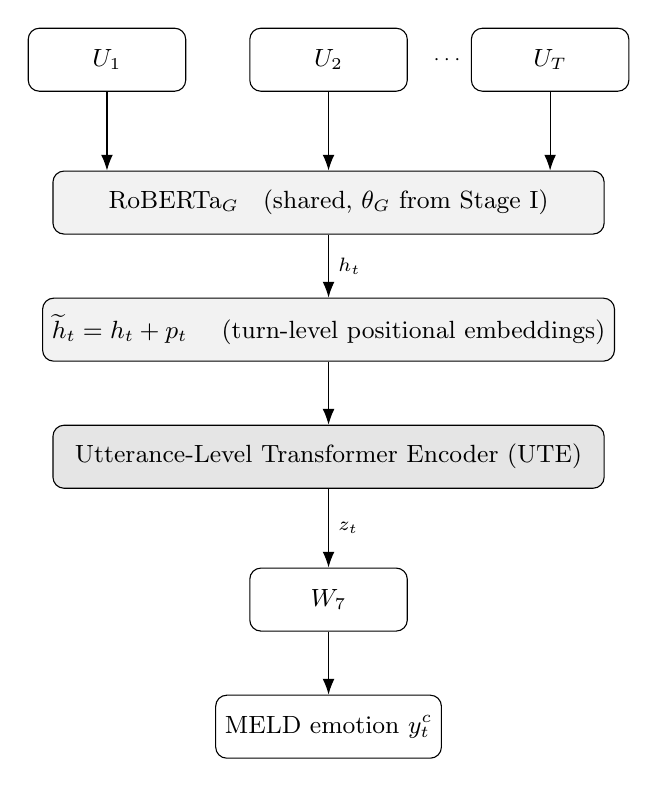
\begin{tikzpicture}[
  node distance=8mm,
  box/.style={draw, rounded corners, minimum height=8mm, minimum width=20mm, font=\small},
  small/.style={font=\scriptsize},
  arrow/.style={-{Latex[length=2mm]}}
]
\node[box] (u1) {$U_1$};
\node[box, right=of u1] (u2) {$U_2$};
\node[box, right=of u2] (ut) {$U_T$};
\node[small, right=2mm of u2] {$\cdots$};

\node[box, fill=black!5, below=10mm of u2, minimum width=70mm] (rob)
  {RoBERTa$_G$ \; (shared, $\theta_G$ from Stage I)};

\node[box, below=8mm of rob, minimum width=70mm, fill=black!5] (pos)
  {$\widetilde{h}_t = h_t + p_t$ \quad (turn-level positional embeddings)};

\node[box, below=8mm of pos, minimum width=70mm, fill=black!10] (ute)
  {Utterance-Level Transformer Encoder (UTE)};

\node[box, below=10mm of ute] (w7) {$W_7$};
\node[box, below=8mm of w7] (out) {MELD emotion $y^c_t$};

\draw[arrow] (u1) -- (u1 |- rob.north);
\draw[arrow] (u2) -- (u2 |- rob.north);
\draw[arrow] (ut) -- (ut |- rob.north);
\draw[arrow] (rob) -- node[right, small] {$h_t$} (pos);
\draw[arrow] (pos) -- (ute);
\draw[arrow] (ute) -- node[right, small] {$z_t$} (w7);
\draw[arrow] (w7) -- (out);
\end{tikzpicture}
\caption{Stage-II architecture. Systems M$_1$ and M$_2$ remove the UTE block and classify
each utterance independently; systems M$_1$ and M$_3$ start from RoBERTa-base instead of
RoBERTa$_G$.}
\label{fig:architecture}
\end{figure}

\subsection{Research extension}
The transfer in $M_4$ is implicit: only the encoder parameters cross between stages, and
the fine-grained predictions themselves are thrown away. The extension tests whether making
them explicit helps. The Stage-I head is retained as a \emph{frozen} predictor, producing a
fine-grained distribution $p^f_t \in \mathbb{R}^{27}$ for every utterance. This is
concatenated with the utterance representation,
\[
e_t = [h_t ; p^f_t] \in \mathbb{R}^{768 + 27},
\]
linearly projected back to $\mathbb{R}^{768}$, and the resulting sequence is processed by
the UTE exactly as before. Only the projection is newly introduced; the rest of the
architecture is identical to $M_4$, so any difference is attributable to the explicit
fine-grained signal.

\section{Experimental Design}

\subsection{Datasets and preprocessing}
GoEmotions contributes 24{,}820 / 3{,}122 / 3{,}154 single-label examples over 27
categories (Section~3.1). MELD contributes 9{,}989 / 1{,}109 / 2{,}610 utterances grouped
into 1{,}038 / 114 / 281 dialogue windows, over seven coarse categories. The class
distribution is heavily skewed: in the training split \texttt{neutral} accounts for 4{,}710
utterances (47.1\%) against 271 for \texttt{disgust} (2.7\%) and 268 for \texttt{fear}
(2.7\%). Dialogue boundaries and utterance order are preserved; dialogues longer than
$T_{\max} = 24$ turns are split into consecutive non-overlapping windows, so every turn is
used and no window spans two dialogues. Utterances are tokenised to at most 64 word pieces.

\subsection{Systems}
\begin{align*}
M_1 &: \mathrm{RoBERTa}_{base} \rightarrow \mathrm{MELD},\\
M_2 &: \mathrm{RoBERTa}_G \rightarrow \mathrm{MELD},\\
M_3 &: \mathrm{RoBERTa}_{base} + \mathrm{UTE} \rightarrow \mathrm{MELD},\\
M_4 &: \mathrm{RoBERTa}_G + \mathrm{UTE} \rightarrow \mathrm{MELD}.
\end{align*}

\subsection{Hyperparameters and protocol}
All systems use AdamW with linear warmup and decay, gradient clipping at 1.0, dropout 0.1,
and weight decay 0.01. Stage~I trains for 4 epochs at learning rate $2\times10^{-5}$ with
batch size 32. Stage~II uses a lower rate for the pretrained backbone
($1\times10^{-5}$) than for the newly initialised UTE and classifier
($1\times10^{-4}$): $M_1$ and $M_2$ train for 5 epochs over batches of 32 utterances,
$M_3$ and $M_4$ for 6 epochs over batches of 4 dialogues. The UTE has 2 layers, 8 heads,
feed-forward width 2048, and learned turn-level positional embeddings. Mixed precision is
used on CUDA only. Every configuration is stored with its run in
\texttt{results/<run>/metrics.json}. Checkpoint selection is by validation (dev) macro-F1;
the test set is used exactly once per system, for the reported numbers. Each system is
trained under three seeds ($42$, $1$, $2$) and results are reported as mean $\pm$ standard
deviation. Every seed also retrains its own Stage-I backbone, so the transfer systems
$M_2$ and $M_4$ inherit a $\theta_G$ matched to their seed rather than sharing one; this
keeps the variance of the transfer arm comparable to that of the baseline arm.

\subsection{Evaluation metrics}
Accuracy, macro-F1 and weighted-F1, with per-class precision, recall and F1. MELD is
class-imbalanced, so macro-F1 is the primary metric.

\section{Results and Analysis}
\begin{table*}[t]
\centering
\caption{MELD test results for the required systems (\%). Mean $\pm$ standard deviation over 3 seeds.}
\label{tab:main}
\begin{tabular}{lccrccc}
\toprule
Model & GoEmotions & UTE & Runs & Accuracy & Macro-F1 & Weighted-F1 \\
\midrule
$M_1$ & No & No & 3 & 65.10 $\pm$ 0.20 & 45.16 $\pm$ 0.34 & 63.74 $\pm$ 0.22 \\
$M_2$ & Yes & No & 3 & 64.96 $\pm$ 0.39 & 47.01 $\pm$ 0.99 & 63.75 $\pm$ 0.46 \\
$M_3$ & No & Yes & 3 & 63.84 $\pm$ 0.25 & 46.31 $\pm$ 0.50 & 63.31 $\pm$ 0.16 \\
$M_4$ & Yes & Yes & 3 & 64.25 $\pm$ 1.00 & 47.65 $\pm$ 0.93 & 63.48 $\pm$ 0.29 \\
ext. & Yes & Yes & 3 & 64.53 $\pm$ 0.29 & 47.57 $\pm$ 0.31 & 63.92 $\pm$ 0.23 \\
\bottomrule
\end{tabular}
\end{table*}


Stage~I reaches $0.5825 \pm 0.0076$ macro-F1 and $0.6574$ accuracy on the GoEmotions test
split under the 27-class single-label reduction described in Section~3.1.

Table~\ref{tab:main} reports the Stage-II results. Because the differences between systems
are of the same order as the spread across seeds, we also compute \emph{paired} per-seed
differences, in which each system is compared against another system trained with the same
seed; this cancels the shared seed effect and is the more informative view.

\begin{table*}[t]
\centering
\caption{Paired per-seed differences in MELD test macro-F1 (points). Each column is one
seed; a comparison is meaningful only if its sign is stable across all three.}
\label{tab:paired}
\begin{tabular}{llrrrr}
\toprule
Comparison & Effect & $s{=}42$ & $s{=}1$ & $s{=}2$ & Mean \\
\midrule
$M_1 \rightarrow M_2$ & fine-grained transfer            & $+1.53$ & $+2.63$ & $+1.38$ & $+1.85$ \\
$M_1 \rightarrow M_3$ & sequential context               & $+1.19$ & $+1.29$ & $+0.97$ & $+1.15$ \\
$M_3 \rightarrow M_4$ & transfer given context           & $+2.25$ & $+0.77$ & $+0.99$ & $+1.34$ \\
$M_1 \rightarrow M_4$ & both                             & $+3.44$ & $+2.07$ & $+1.96$ & $+2.49$ \\
\midrule
$M_4 \rightarrow$ ext. & explicit $p^f_t$                & $-1.28$ & $+0.37$ & $+0.66$ & $-0.08$ \\
\bottomrule
\end{tabular}
\end{table*}

\paragraph{$M_1$ vs $M_2$: fine-grained transfer.}
Transferring the GoEmotions-trained backbone improves macro-F1 by $1.85$ points, positive
in all three seeds. Per class, the effect is almost entirely confined to the two rarest
categories: \texttt{disgust} improves by $0.122$ F1 and \texttt{fear} by $0.070$, while
the frequent categories move by less than $0.01$ in either direction. This is consistent
with the intuition behind the design --- MELD supplies too few \texttt{disgust} and
\texttt{fear} examples ($271$ and $268$ in training) to learn these categories from
scratch, and the fine-grained corpus supplies the missing signal.

\paragraph{$M_1$ vs $M_3$: sequential context.}
Adding the UTE without transfer improves macro-F1 by $1.15$ points, again positive in every
seed, with gains for \texttt{disgust} ($+0.067$), \texttt{fear} ($+0.039$),
\texttt{anger} and \texttt{sadness}. Unlike transfer, context costs something on the
frequent classes: \texttt{neutral} loses $0.015$ F1 and \texttt{surprise} $0.019$, and
overall accuracy falls from $0.6510$ to $0.6384$. The sequence model redistributes
probability mass away from the majority class, which is precisely why macro-F1 rises while
accuracy does not.

\paragraph{$M_3$ vs $M_4$: does transfer still help once context is modelled?}
Yes. Adding the transferred backbone on top of the UTE improves macro-F1 by a further
$1.34$ points, positive in all three seeds, and the largest single per-class gain in the
whole study appears here: \texttt{fear} improves by $0.090$ F1. The two effects therefore
do not merely overlap. Their combination, $M_1 \rightarrow M_4$, yields $+2.49$ macro-F1,
which is close to the sum of the individual effects and is positive in every seed.

\paragraph{Extension: explicit fine-grained distribution.}
Concatenating the frozen Stage-I distribution $p^f_t$ with the utterance representation
does not improve macro-F1: the mean difference against $M_4$ is $-0.08$ points and the sign
is not stable across seeds. The extension does achieve the best weighted-F1 of any system
($0.6392$) and the smallest variance, so it trades minority-class recall for stability on
the frequent classes. We read this as evidence that what transfers usefully between stages
is the \emph{representation} shaped by fine-grained training, not the fine-grained label
predictions.

\paragraph{Accuracy versus macro-F1.}
Accuracy is flat to slightly negative across the whole study while macro-F1 rises
monotonically. This is expected rather than anomalous: \texttt{neutral} accounts for
$48.1\%$ of the test utterances, so accuracy is dominated by a class on which all systems
already score around $0.78$--$0.80$ F1, and every improvement reported here is bought from
the rare classes.

\section{Error Analysis}
All examples below are drawn from \path{docs/tables/error_analysis.json}, which is
generated from the saved test predictions.

\paragraph{Where context changes the interpretation.}
The clearest cases are short utterances whose emotion is fixed entirely by the preceding
turn. In dialogue 4, the utterance \emph{``What?''} follows \emph{``Ohh!''} and is labelled
\texttt{neutral}; the context-free $M_2$ predicts \texttt{surprise} from the question form
alone, while $M_4$ reads the exclamation as already carrying the surprise and predicts
\texttt{neutral}. The reverse pattern also occurs: \emph{``Bumpy?''}, following
\emph{``It was just so awkward and bumpy''}, is genuinely \texttt{surprise}, which $M_4$
recovers and $M_2$ misses. Longer-range cases exist too --- \emph{``I mean there's no way
Joey's gonna make it in time''} is labelled \texttt{fear} and predicted as \texttt{sadness}
without context, but correctly with the preceding \emph{``we gotta do something!''}.

\paragraph{Where context hurts.}
Every case in which the context-free system wins and the sequential system loses occurs at a
\emph{dialogue-initial} turn, where the UTE has no previous utterance to condition on. The
repeated exclamation \emph{``Push!''} (labelled \texttt{joy}) is predicted correctly by
$M_2$ and as \texttt{anger} by $M_4$: with an empty left context the sequence model appears
to fall back on the lexical intensity of the utterance. This suggests the UTE is not merely
smoothing predictions but is genuinely dependent on the availability of context.

\paragraph{Where fine-grained transfer helps.}
Transfer resolves cases that require distinguishing between negative emotions of similar
valence. \emph{``Oh wait, Joey, you can't go like that! You stink!''} is labelled
\texttt{disgust} and predicted as \texttt{anger} by $M_3$ but correctly by $M_4$. The
GoEmotions taxonomy contains \texttt{disgust}, \texttt{annoyance} and \texttt{anger} as
separate categories, so the transferred encoder has been trained to separate exactly this
distinction, which MELD alone provides too few examples to teach.

\paragraph{Dominant confusions.}
Across all systems the largest off-diagonal cells involve \texttt{neutral}:
\texttt{neutral} $\rightarrow$ \texttt{joy} ($84$--$98$ utterances depending on the system),
\texttt{joy} $\rightarrow$ \texttt{neutral} ($\approx 76$) and
\texttt{sadness} $\rightarrow$ \texttt{neutral} ($\approx 71$--$79$). The
\texttt{neutral}/\texttt{joy} boundary is the single hardest distinction in the corpus,
which is unsurprising for a situation comedy in which conversational filler is delivered
cheerfully. Note that the sequential systems shift \emph{more} mass into
\texttt{neutral} $\rightarrow$ \texttt{joy} errors, which is where their accuracy loss
originates.

\paragraph{The remaining failure mode.}
Even the best system reaches only $0.26$ F1 on \texttt{fear} and $0.28$ on
\texttt{disgust}. With $50$ and $68$ test utterances respectively, these classes are both
hard to learn and noisy to measure --- a handful of predictions moves their F1 by several
points, which is also why they dominate the seed variance in Table~\ref{tab:main}.

\section{Conclusion}

\paragraph{Implemented work.}
A complete two-stage pipeline: Stage-I fine-tuning of RoBERTa-base on 27 fine-grained
GoEmotions categories with the classification head discarded afterwards; Stage-II transfer
of the backbone to MELD with turn-level positional embeddings, an utterance-level
Transformer encoder and a new 7-class head, with all three components trainable; the four
required systems $M_1$--$M_4$ and the fine-grained-distribution extension; and an evaluation
harness producing accuracy, macro-F1, weighted-F1, per-class scores, confusion matrices and
contrastive error analysis. Dialogue boundaries and utterance order are preserved
throughout, and the test set is used once per system.

\paragraph{Experimental findings.}
Fine-grained transfer and sequential context both improve coarse-grained emotion
recognition on MELD, and they combine: $+1.85$ and $+1.15$ macro-F1 points individually,
$+2.49$ together, each positive in all three seeds. The answer to the research question is
therefore affirmative --- fine-grained emotion learning still contributes after dialogue
context is modelled ($M_3 \rightarrow M_4$, $+1.34$). The gains are concentrated in the
rare \texttt{disgust} and \texttt{fear} categories and are paid for by a small loss on
\texttt{neutral}, so accuracy does not improve even though macro-F1 does. Making the
fine-grained predictions explicit in the sequence input does not help further.

\paragraph{Limitations.}
The study is text-only, while MELD also provides audio and video. Dialogues longer than
$T_{\max} = 24$ turns are split into windows, so context does not cross a window boundary.
Three seeds establish the direction of each effect but do not constitute a significance
test, and no such test is claimed. Model selection uses dev macro-F1 with a fixed
hyperparameter configuration rather than a search, so the absolute numbers are not tuned
ceilings. Finally, MELD is drawn from a single television series, which limits how far the
conclusions generalise to other conversational domains.

\paragraph{Future work.}
Three directions follow directly from the findings. First, since the gains are
minority-class gains, combining transfer with class-balanced or focal losses should compound
them. Second, the failure of the explicit-distribution extension suggests the fine-grained
signal is better injected during training --- for instance by multi-task training on both
label sets --- than concatenated at inference. Third, the dialogue-initial failures of the
UTE suggest speaker-aware conditioning or a causal attention mask, both of which the current
implementation supports behind flags but which were not evaluated here.

\balance
\bibliographystyle{ACM-Reference-Format}
\bibliography{report}

\end{document}
